\section{Contact Angle Measurement}

The water contact angle (\gls{WCA}) is the standard characterization method 
used in the optical contact bonding literature to assess the chemical 
state of a glass surface prior to bonding \cite{gosele2006, possl1999}. 
In this simple method, the measured angle is a direct proxy for 
the density of reactive surface groups that govern bond formation.

The contact angle $\theta_C$ is geometrically defined as the angle 
formed at the three-phase boundary where a liquid droplet, the 
surrounding gas, and the solid substrate meet simultaneously, as 
illustrated in Figure~\ref{fig:contact_angle_definition}. At mechanical 
equilibrium, the angle satisfies Young's equation \cite{degennes2004}:
%
\begin{equation}
    \cos\theta_C = \frac{\gamma_{sg} - \gamma_{sl}}{\gamma_{lg}},
    \label{eq:young}
\end{equation}
%
where $\gamma_{sg}$, $\gamma_{sl}$, and $\gamma_{lg}$ denote the 
solid--gas, solid--liquid, and liquid--gas interfacial energies, 
respectively. This equation expresses the condition that minimises the 
total free energy of the system for a virtual displacement of the 
contact line \cite{degennes2004}: the contact angle is determined 
entirely by the balance between the tendency of the liquid to spread 
over the solid (governed by $\gamma_{sg} - \gamma_{sl}$) and the 
tendency of the liquid--gas interface to contract (governed by 
$\gamma_{lg}$). As $\gamma_{sg}$ increases relative to $\gamma_{sl}$, 
the liquid spreads more, and $\theta_C$ decreases.

\begin{figure}[h]
\centering
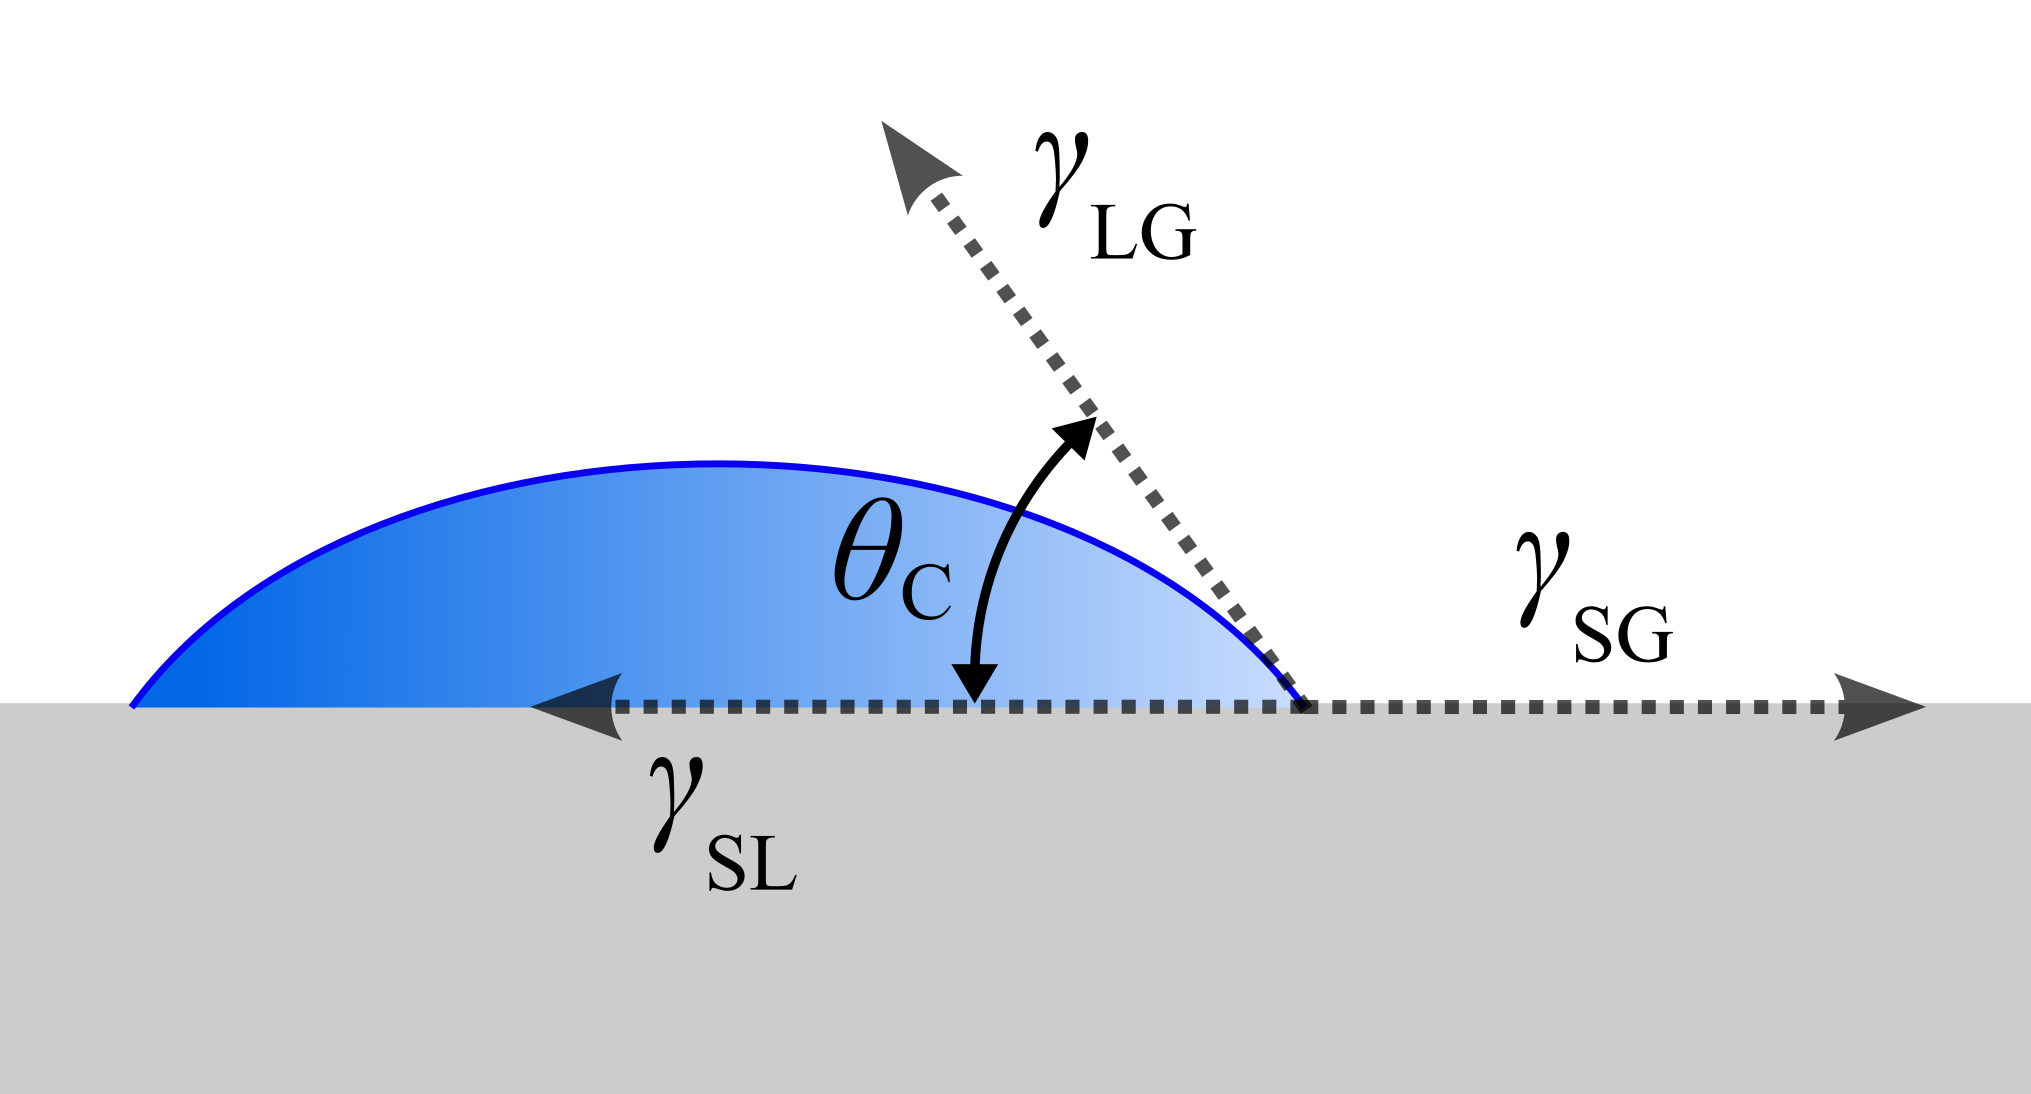
\includegraphics[width=0.6\textwidth]{Images/Contact_angle.png} 
\caption{Geometrical definition of the contact angle $\theta_C$ at the 
    three-phase boundary between a liquid droplet, the ambient gas, and 
    the solid substrate. The equilibrium value is set by the balance of 
    interfacial energies expressed in Young's equation 
    (Eq.~\eqref{eq:young}). From \cite{wikicontact}.}
\label{fig:contact_angle_definition}
\end{figure}

On silica and glass surfaces, the magnitude of $\gamma_{sg}$ is 
controlled by the density of surface hydroxyl groups, commonly 
referred to as silanol groups (Si-OH). Silanol groups are simultaneously 
hydrogen-bond donors and acceptors \cite{zhuravlev2000}, 
which gives them a strong chemical affinity for water. A fully 
hydroxylated silica surface
therefore exhibits a very high $\gamma_{sg}$ and a low $\gamma_{sl}$, 
resulting in low contact angles. As the silanol density decreases, 
whether due to thermal treatment, which converts Si-OH groups into 
hydrophobic siloxane bridges (Si-O-Si), or due to organic contamination, 
which physically blocks hydrophilic sites, $\gamma_{sg}$ falls and 
$\gamma_{sl}$ rises. By Young's equation, this directly translates into 
an increase in $\theta_C$. The WCA thus provides an experimentally accessible 
measurement of the silanol surface density, without requiring the use of 
more complex or expensive techniques.

\begin{figure}[h]
\centering
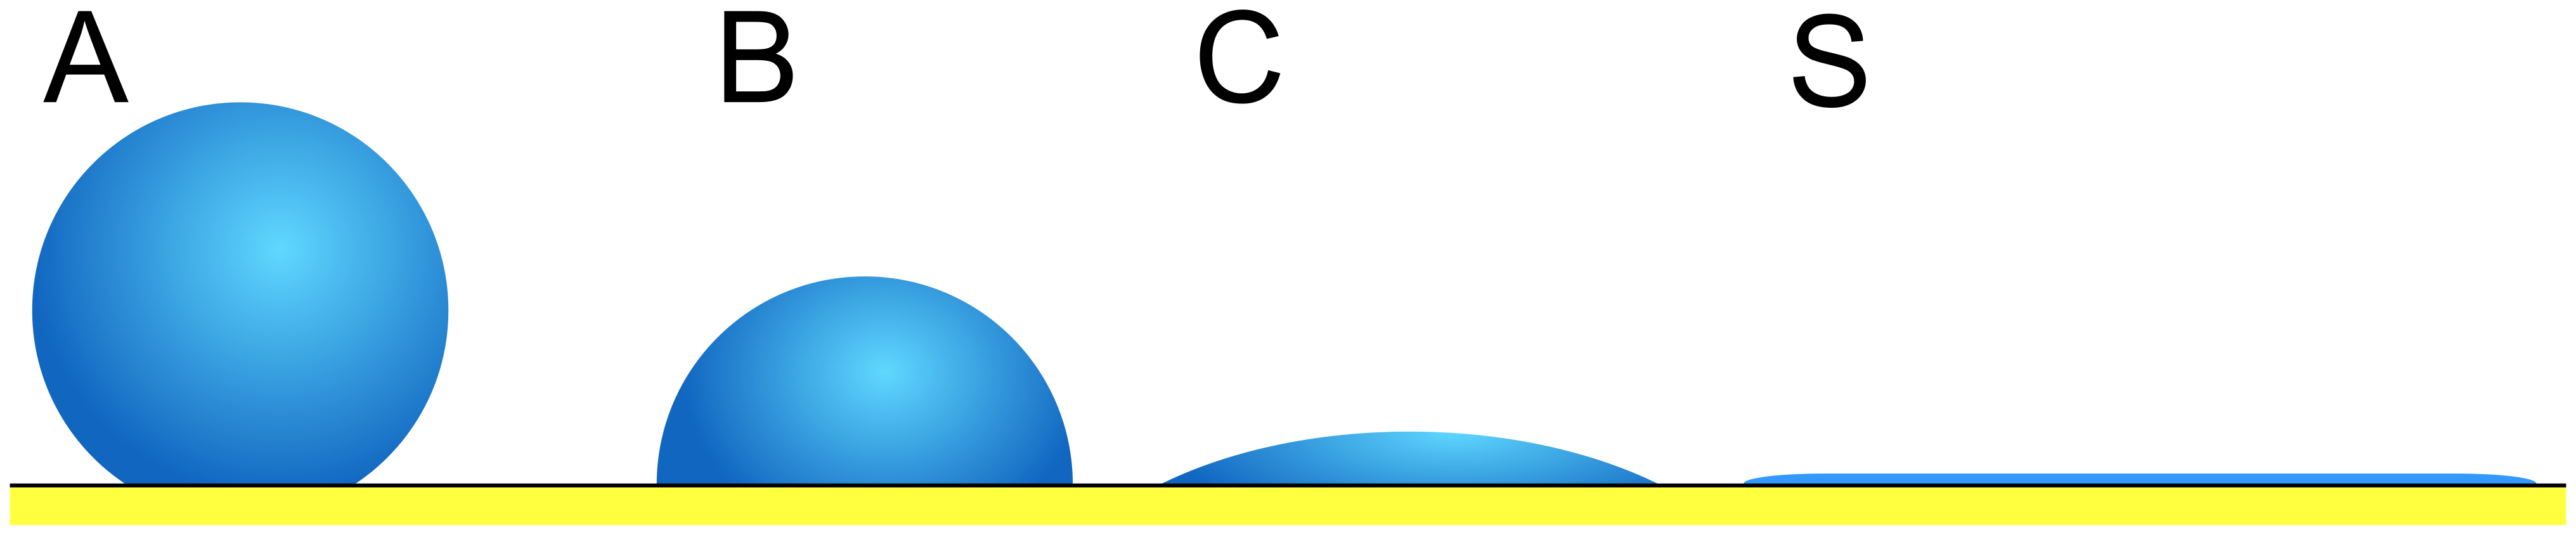
\includegraphics[width=0.7\textwidth]{Images/Surface_tension.png} 
\caption{Representative contact angle regimes across different 
    wettability states. Surface~A ($\theta_C > 90^\circ$) is 
    hydrophobic; surfaces~B, C, and S are sorted from partially to 
    fully hydrophilic ($\theta_C \to 0^\circ$). From \cite{wikicontacts}.}
\label{fig:contact_angles}
\end{figure}

The connection between the WCA and optical contact bonding is therefore 
direct: the silanol groups whose density is encoded in the contact angle 
are the same reactive sites that initiate bond formation. A low 
WCA is therefore not merely a qualitative indicator of surface 
cleanliness, but a quantitative predictor of the maximum achievable bond 
energy. For this reason, a contact angle below $\sim 5^\circ$ is 
consistently used as the pass/fail threshold for surface activation in 
the direct bonding literature \cite{gosele2006, possl1999}.